\chapter{Uso del sistema}
\label{ch:usodelsistema}
Es este capítulo realizaremos un recorrido guiado sobre el uso de nuestra herramienta. Explicaremos paso a paso cada una de las opciones que hay a nuestra disposición y adjuntaremos capturas de pantalla de cada acción realizada. Recordamos que el sistema está disponible en \url{http://browserfingerprinting.educationhost.cloud/}

\section{Bienvenida}

Lo primero que nos encontramos al acceder a la \textit{URL} es una pantalla de bienvenida como la que aparece en la figura \ref{fig:wellcome}. Aquí damos una breve explicación de qué es la huella digital de un navegador web, introducimos en qué consiste nuestro proyecto e informamos al usuario del tratamiento que vamos a hacer con sus datos. Para continuar, pincharemos en el botón \texttt{Ver huella digital de tu navegador}.

\begin{figure}[tbp]
	\centering
	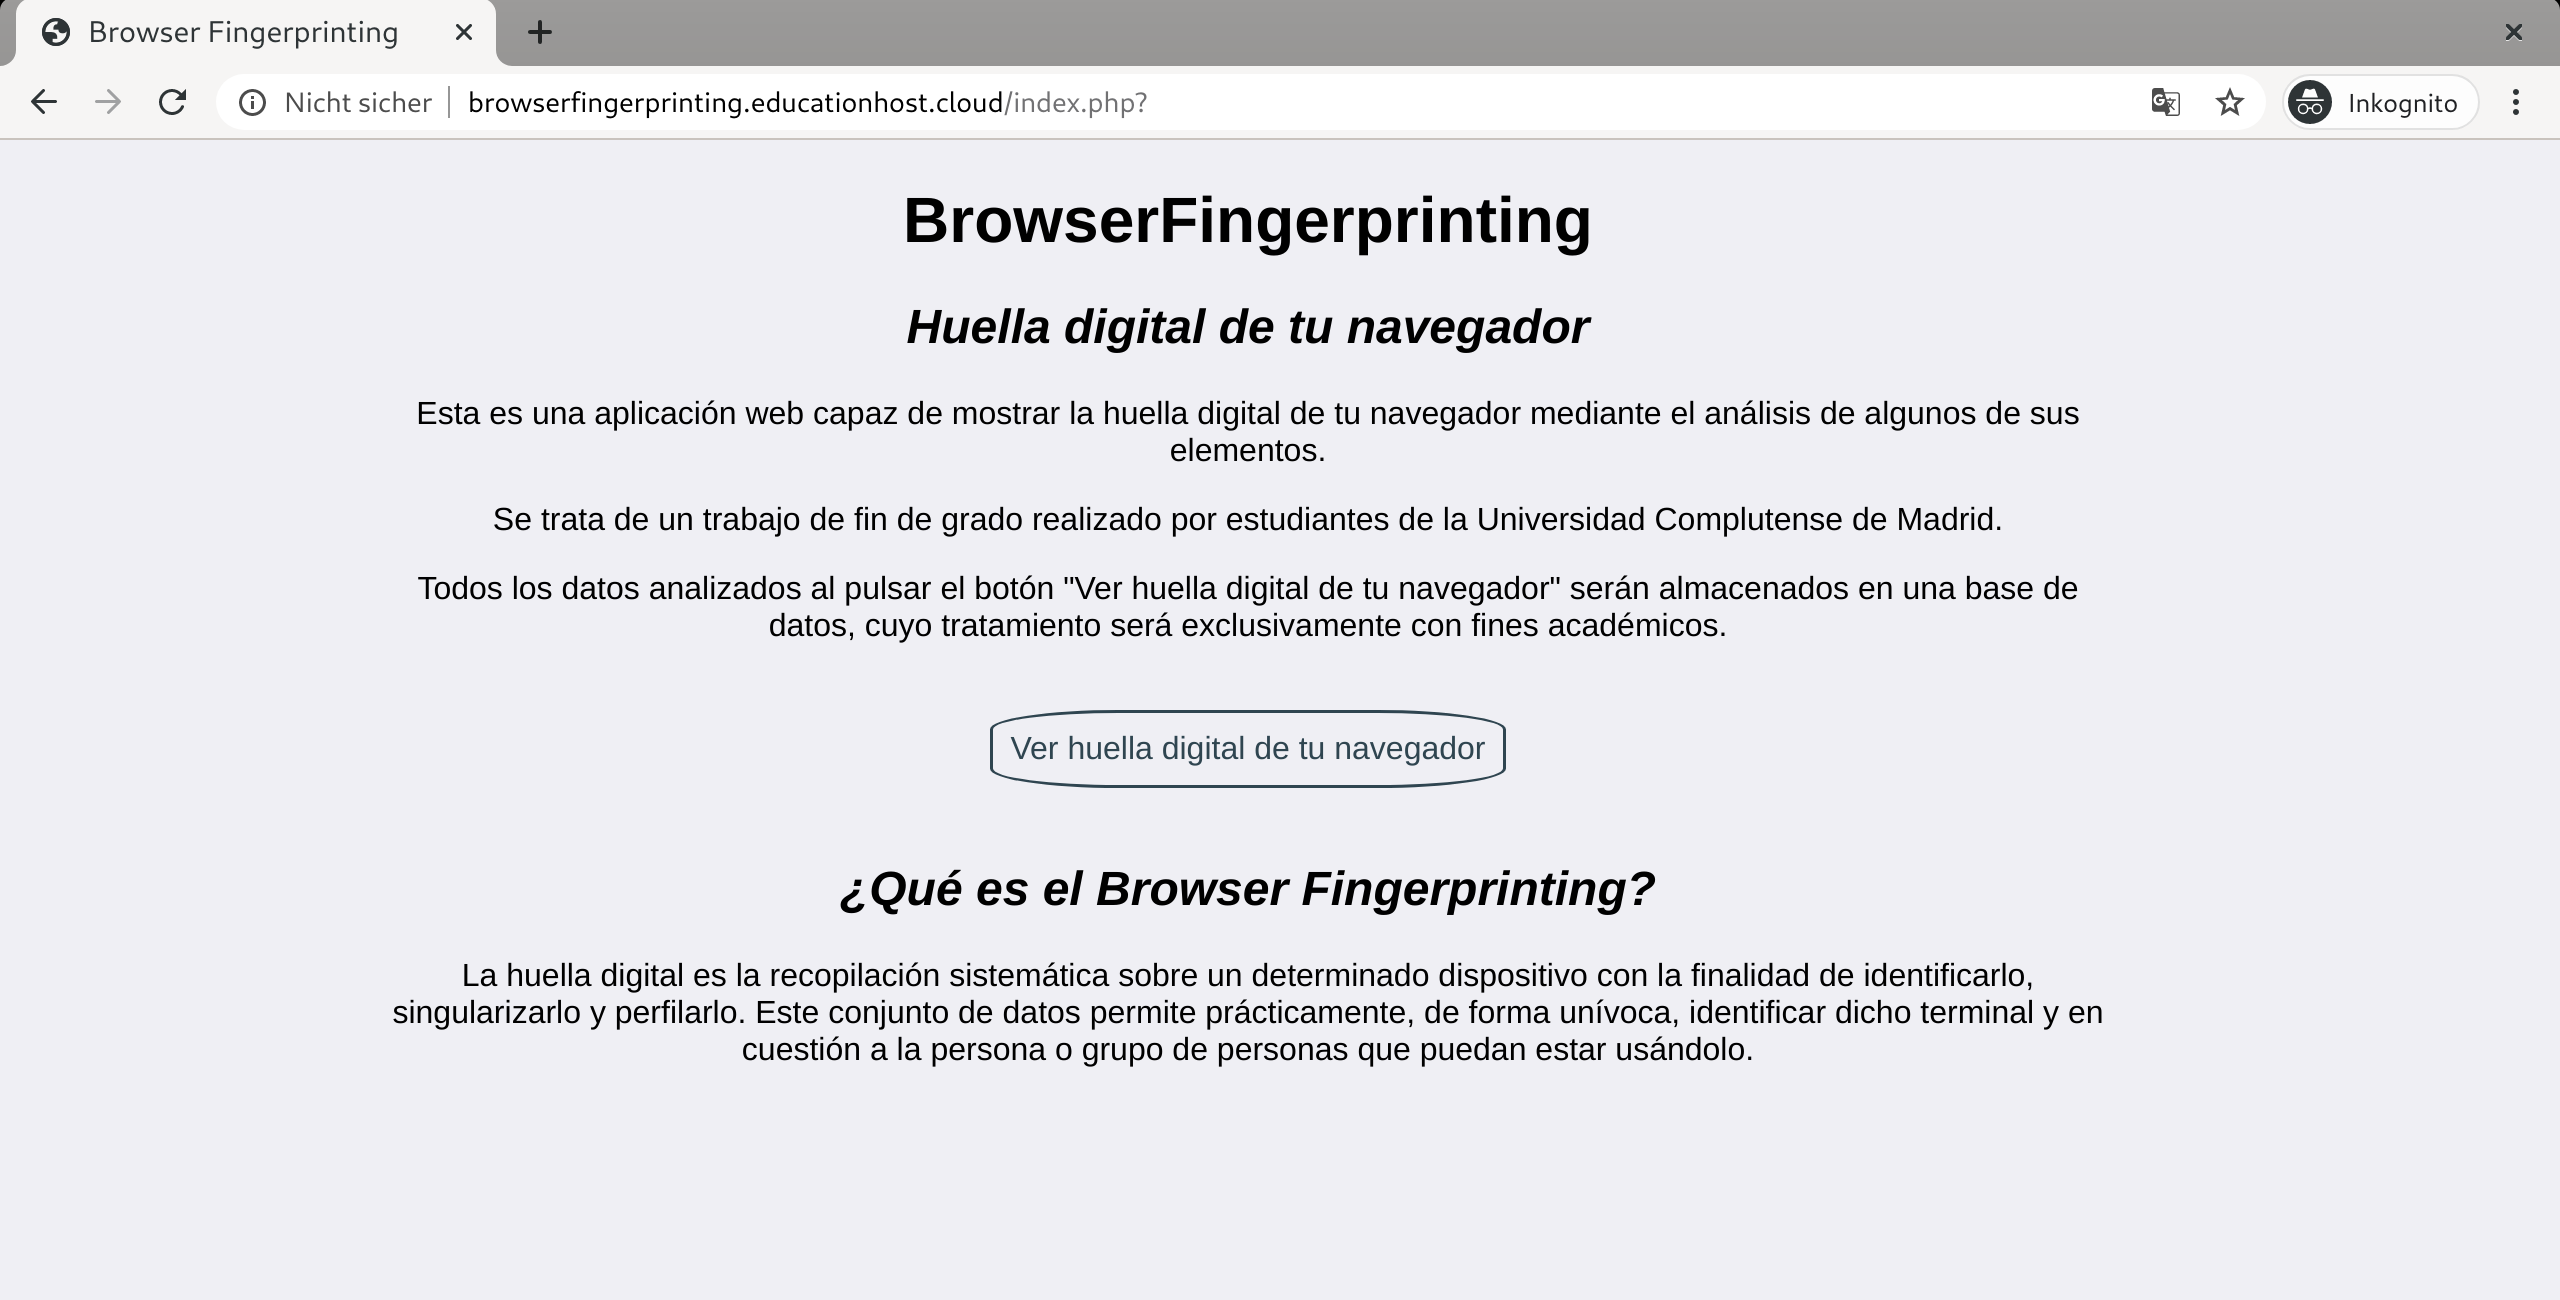
\includegraphics[width=1\textwidth]{Images/wellcome.png}
	\caption{Pantalla de bienvenida.}
	\label{fig:wellcome}
\end{figure}

\section{Índice}

Tras pinchar en el botón de la sección anterior, la página nos carga un índice con distintas secciones. También aparece arriba a la izquierda el botón de \texttt{Gráficos}, que detallaremos en el siguiente apartado.

\subsubsection{Resultado}
La primera de las secciones es la de Resultado, figura \ref{fig:resultadoSection}, que nos indica cuántas huellas digitales iguales a la del usuario se han encontrado en nuestra base de datos. Esto es, nos da el porcentaje de unicidad total del usuario. A partir de aquí se muestran varias secciones con tablas. En cada tabla aparece: \par

\begin{figure}[tbp]
	\centering
	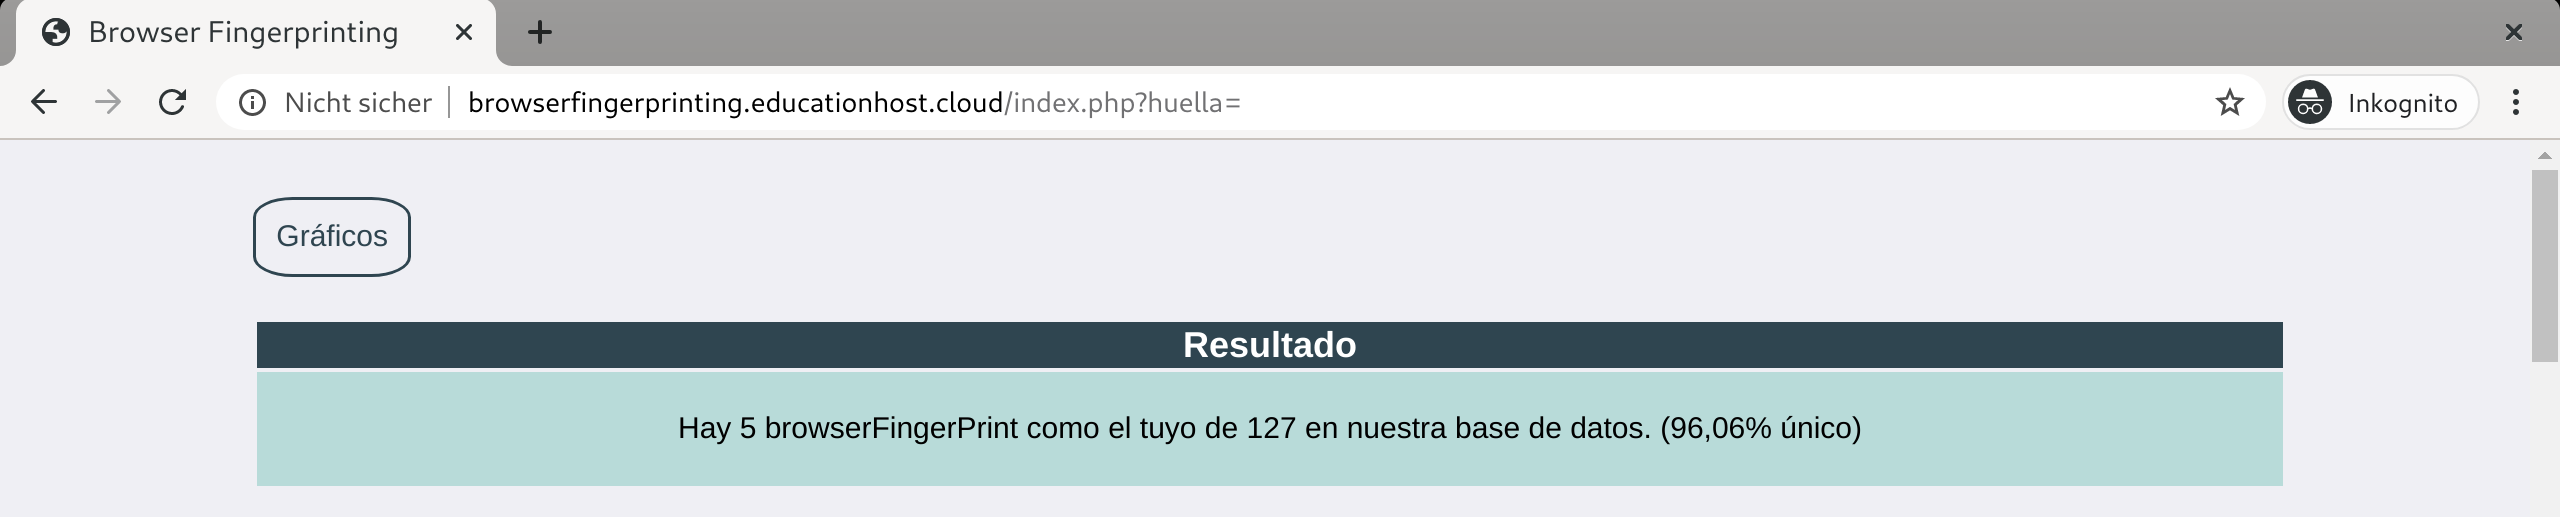
\includegraphics[width=1\textwidth]{Images/resultadoSection.png}
	\caption{Porcentaje de unicidad total.}
	\label{fig:resultadoSection}
\end{figure}

\begin{itemize}
	\item Cada elemento de esa sección.
	\item El porcentaje de similaridad que existe entre el valor del elemento y los que tenemos guardados en la base de datos.
	\item El valor que toma el elemento en nuestro dispositivo.
\end{itemize}

\subsubsection{Cabecera HTTP}
En la figura \ref{fig:headersSection} se nos muestra una tabla con los distintos campos que contiene la cabecera de petición HTTP del cliente. Si situamos el cursor encima del botón \texttt{info} que aparece en cada elemento, podemos leer una pequeña explicación sobre su significado.

\begin{figure}[tbp]
	\centering
	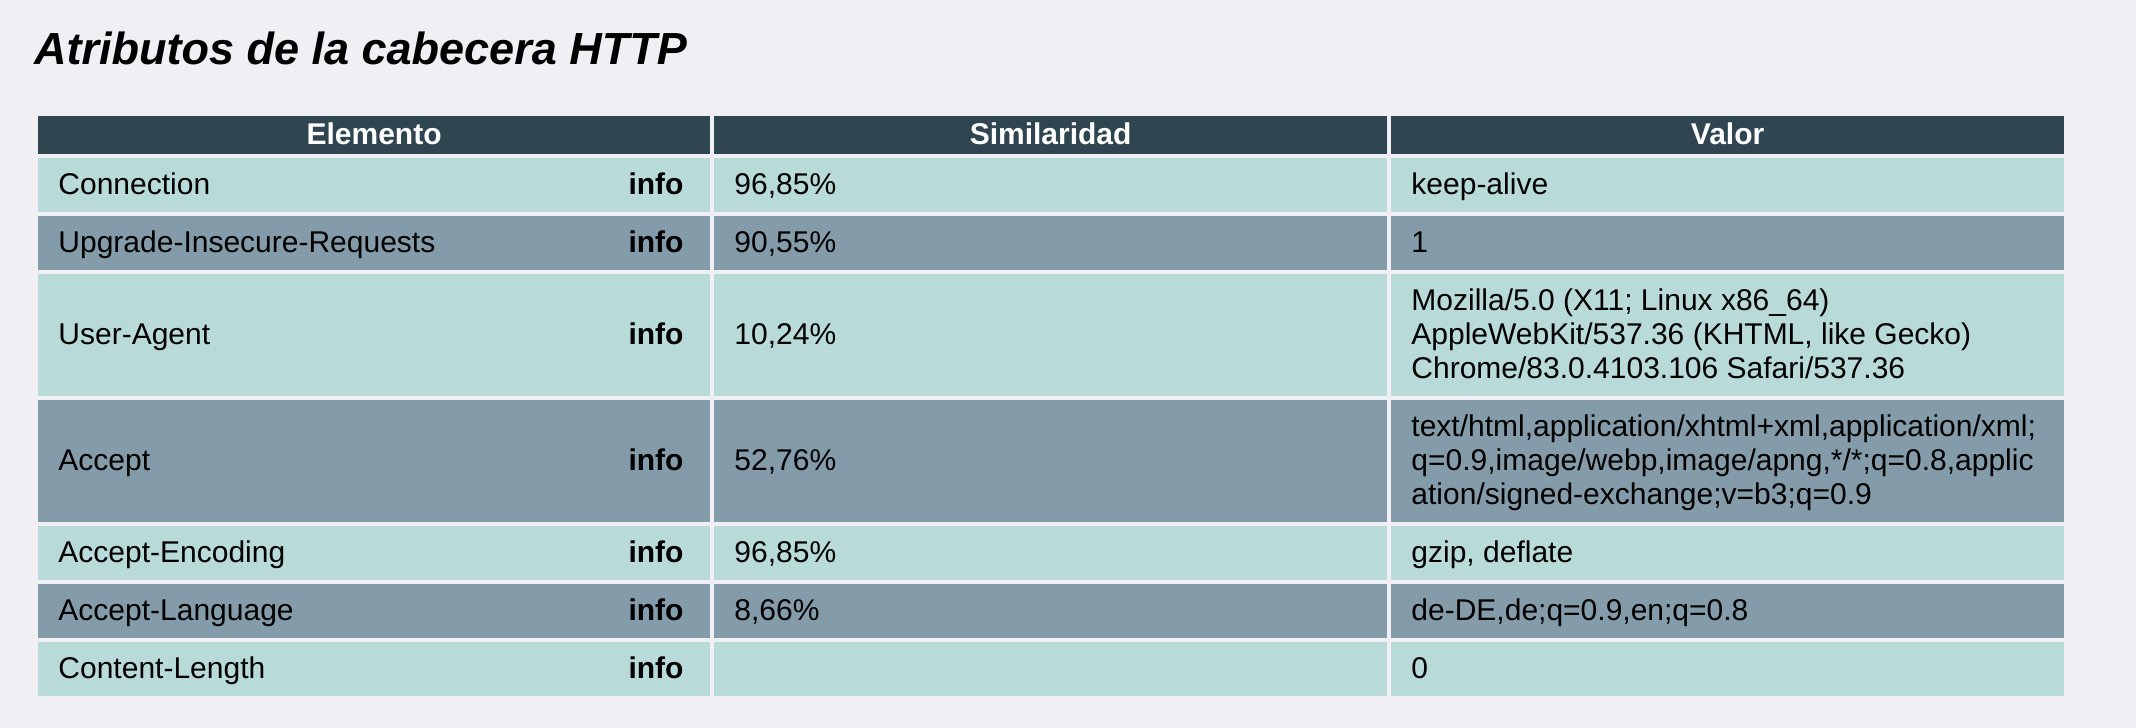
\includegraphics[width=1\textwidth]{Images/headersSection.png}
	\caption{Cabecera HTTP.}
	\label{fig:headersSection}
\end{figure}

\subsubsection{JavaScript}

Aquí mostramos información sobre los elementos a los que accedemos desde WebAPI a través de JavaScript, que se puede observar en la figura \ref{fig:javaScriptSection.png}. En el atributo de \texttt{canvas} pintamos sobre el lienzo del navegador y le mostramos el dibujo al usuario, como se puede ver en la figura \ref{fig:canvas.png}.

\subsubsection{Formatos de vídeo}
Cada navegador es capaz de reproducir unos formatos de vídeo específicos. En la figura \ref{fig:videosSection} se pueden ver los valores que se obtienen. El valor \texttt{probably} indica que es muy probable que dicho formato esté soportado, en cambio el valor \texttt{maybe} nos da una respuesta más incierta. Se realiza esta distinción porque aunque a veces el formato está soportado, algunos códecs en concreto puede que no lo estén. Si el formato no está soportado por el navegador, se muestra el resultado \texttt{No soportado}.

\subsubsection{Formatos de audio}
De forma análoga a los formatos de vídeo, en la figura \ref{fig:audiosSection} mostramos una tabla con los formatos de audio a los que el navegador es capaz de dar soporte.

\begin{figure}[tbp]
	\centering
	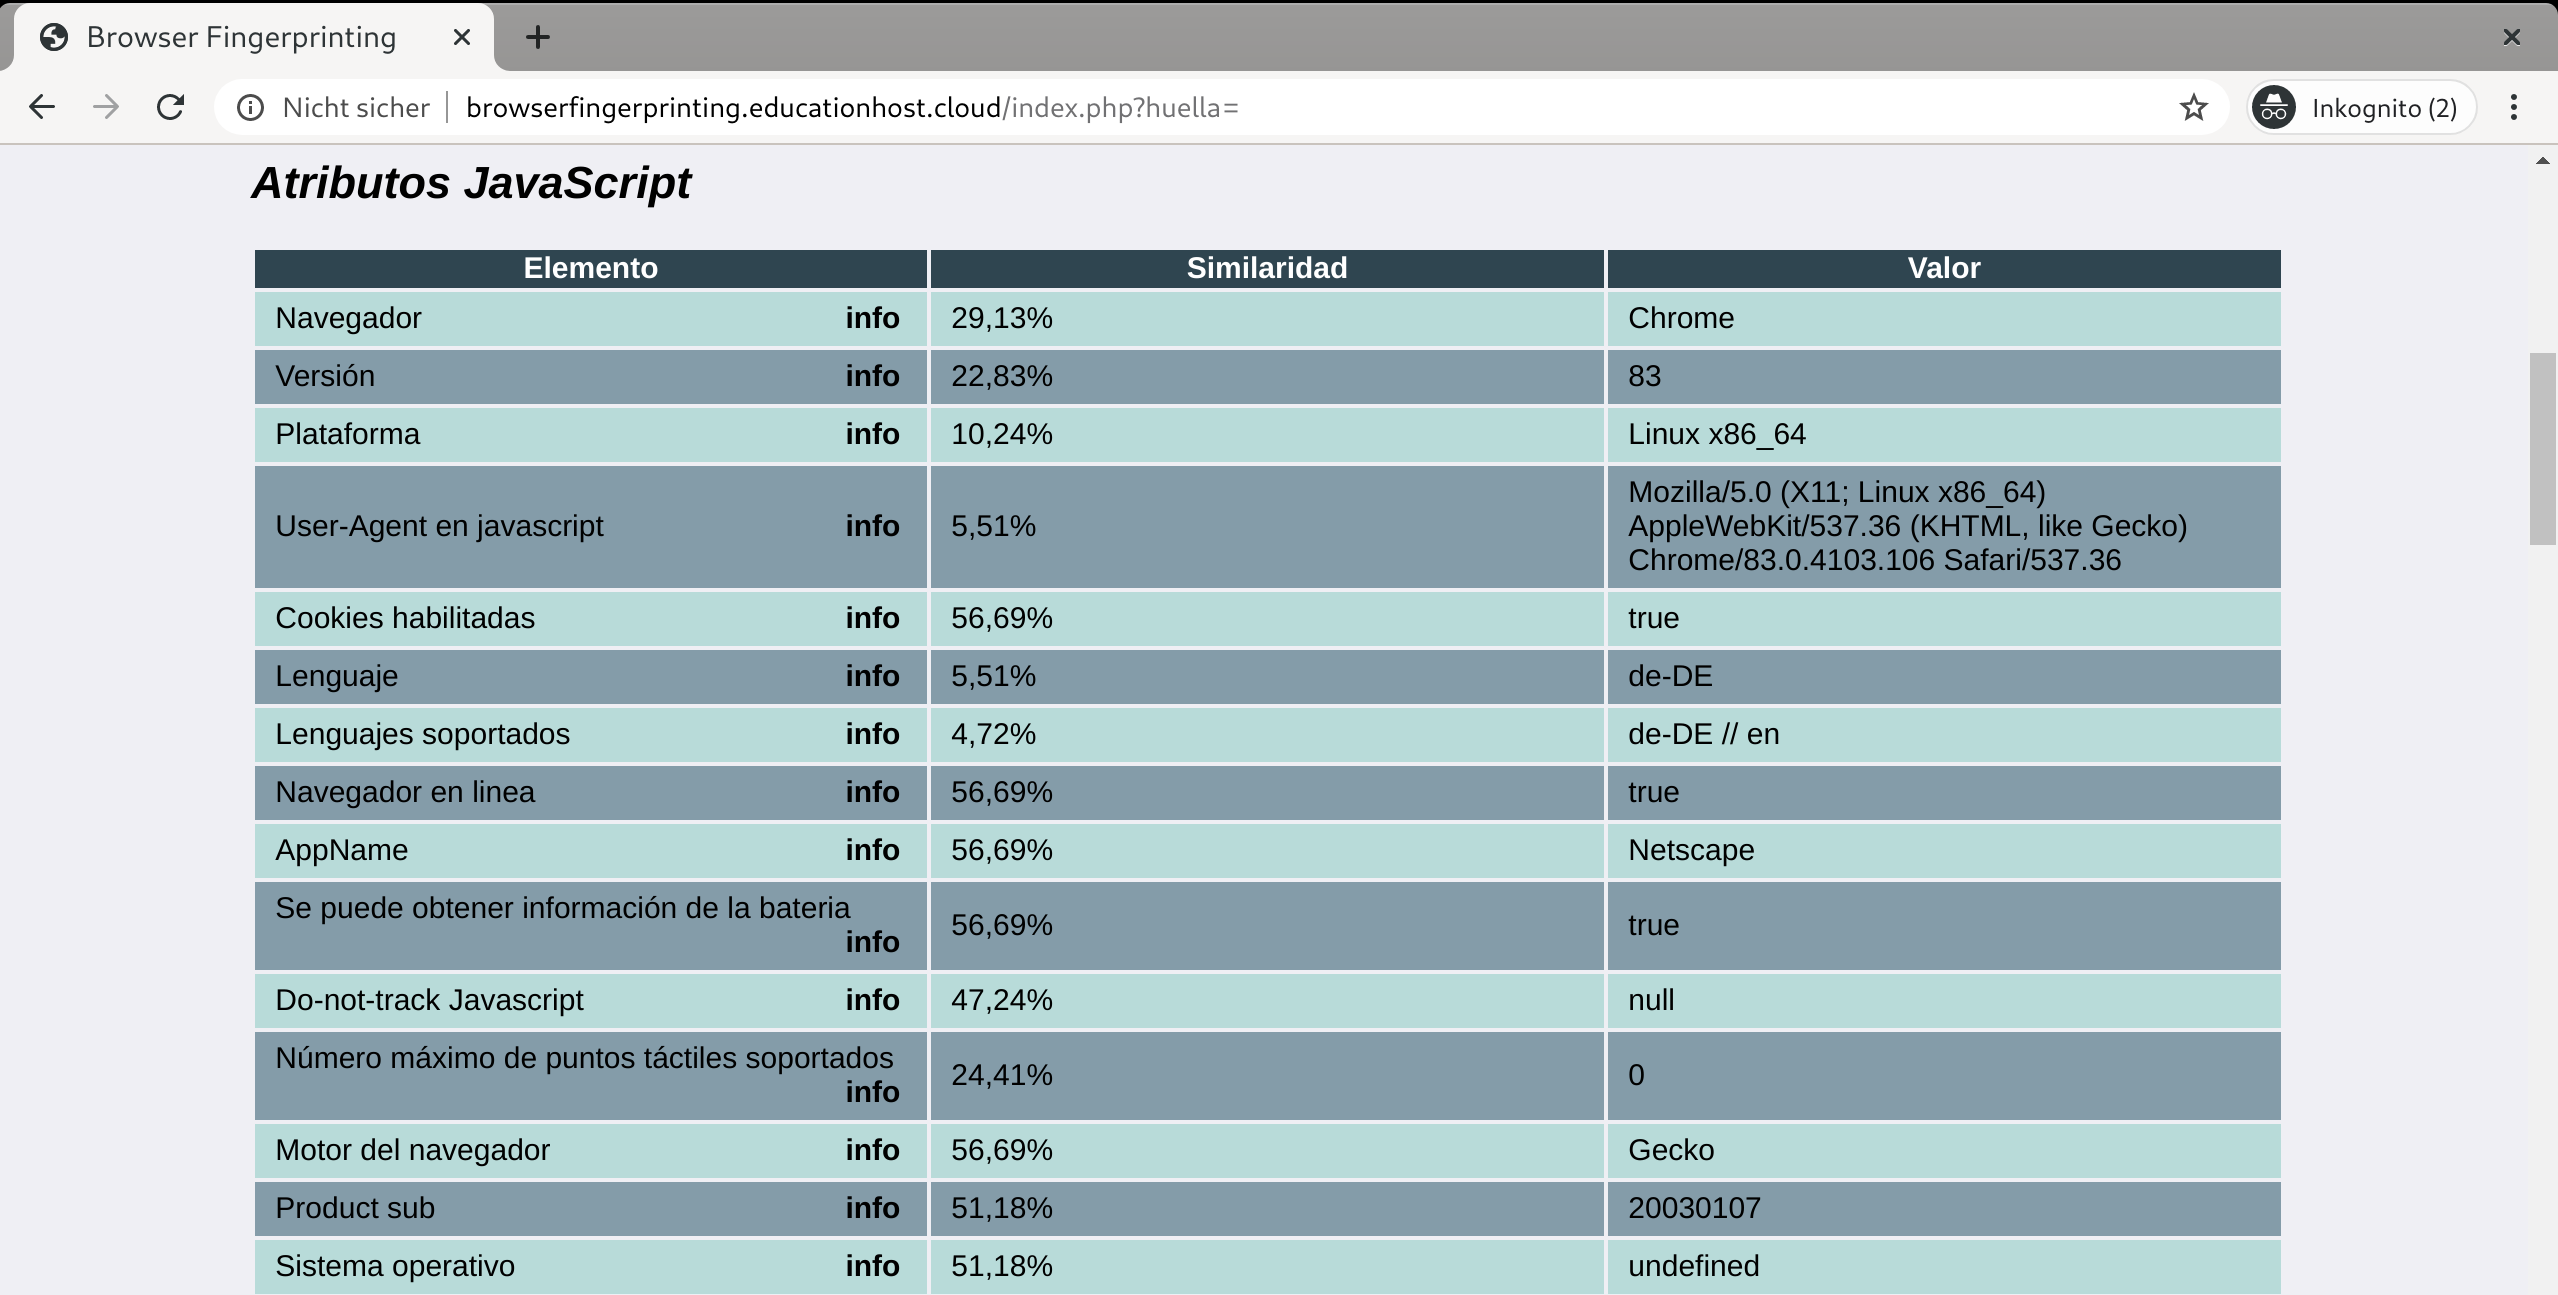
\includegraphics[width=1\textwidth]{Images/javaScriptSection.png}
	\caption{Elementos accedidos desde WebAPI a través de Javascript.}
	\label{fig:javaScriptSection.png}
\end{figure}

\begin{figure}[tbp]
	\centering
	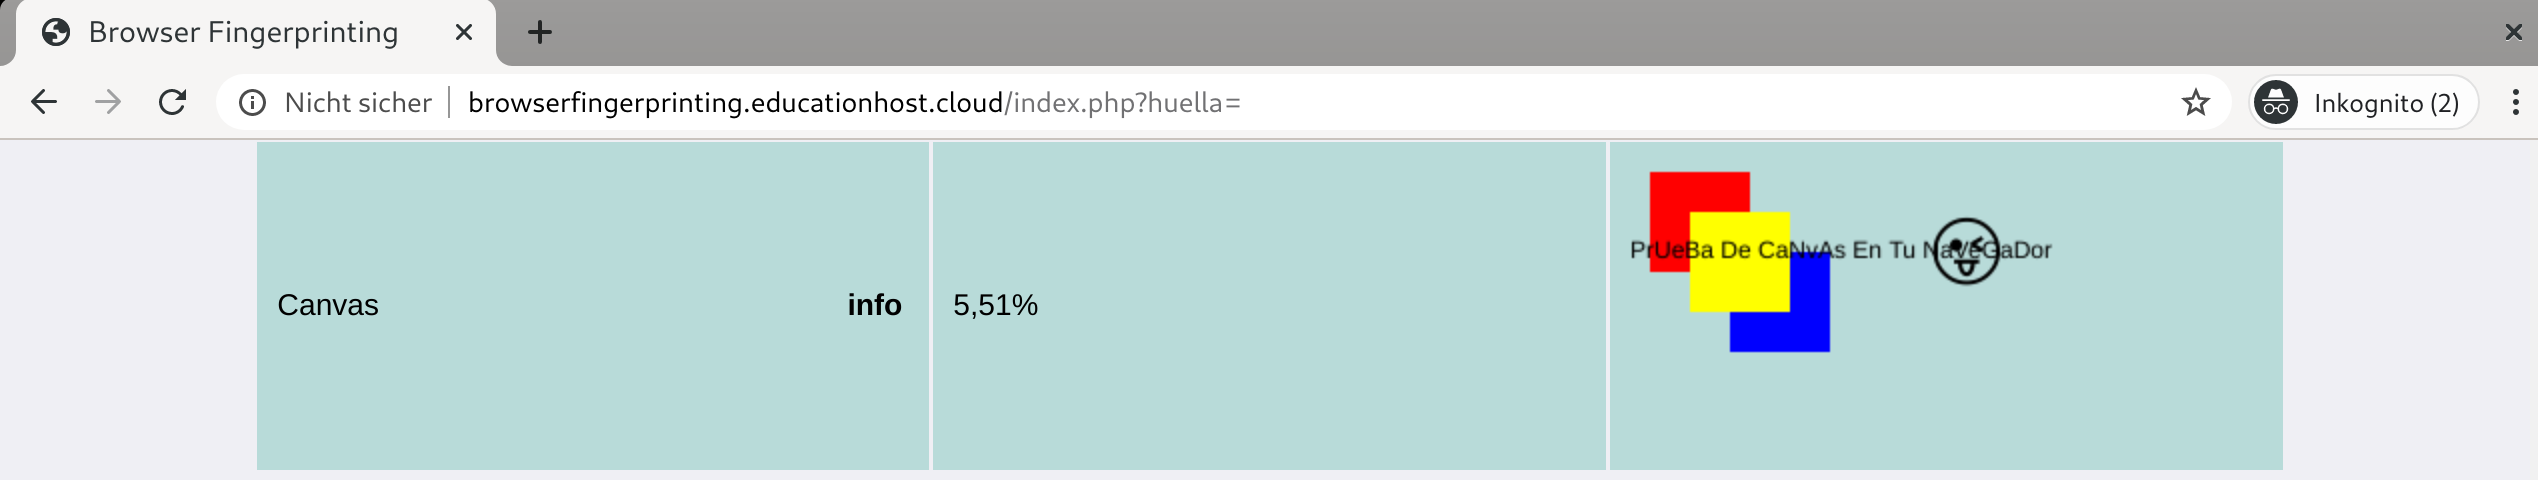
\includegraphics[width=1\textwidth]{Images/canvas.png}
	\caption{Obtención de la huella digital a través del lienzo.}
	\label{fig:canvas.png}
\end{figure}

\begin{figure}[tbp]
	\centering
	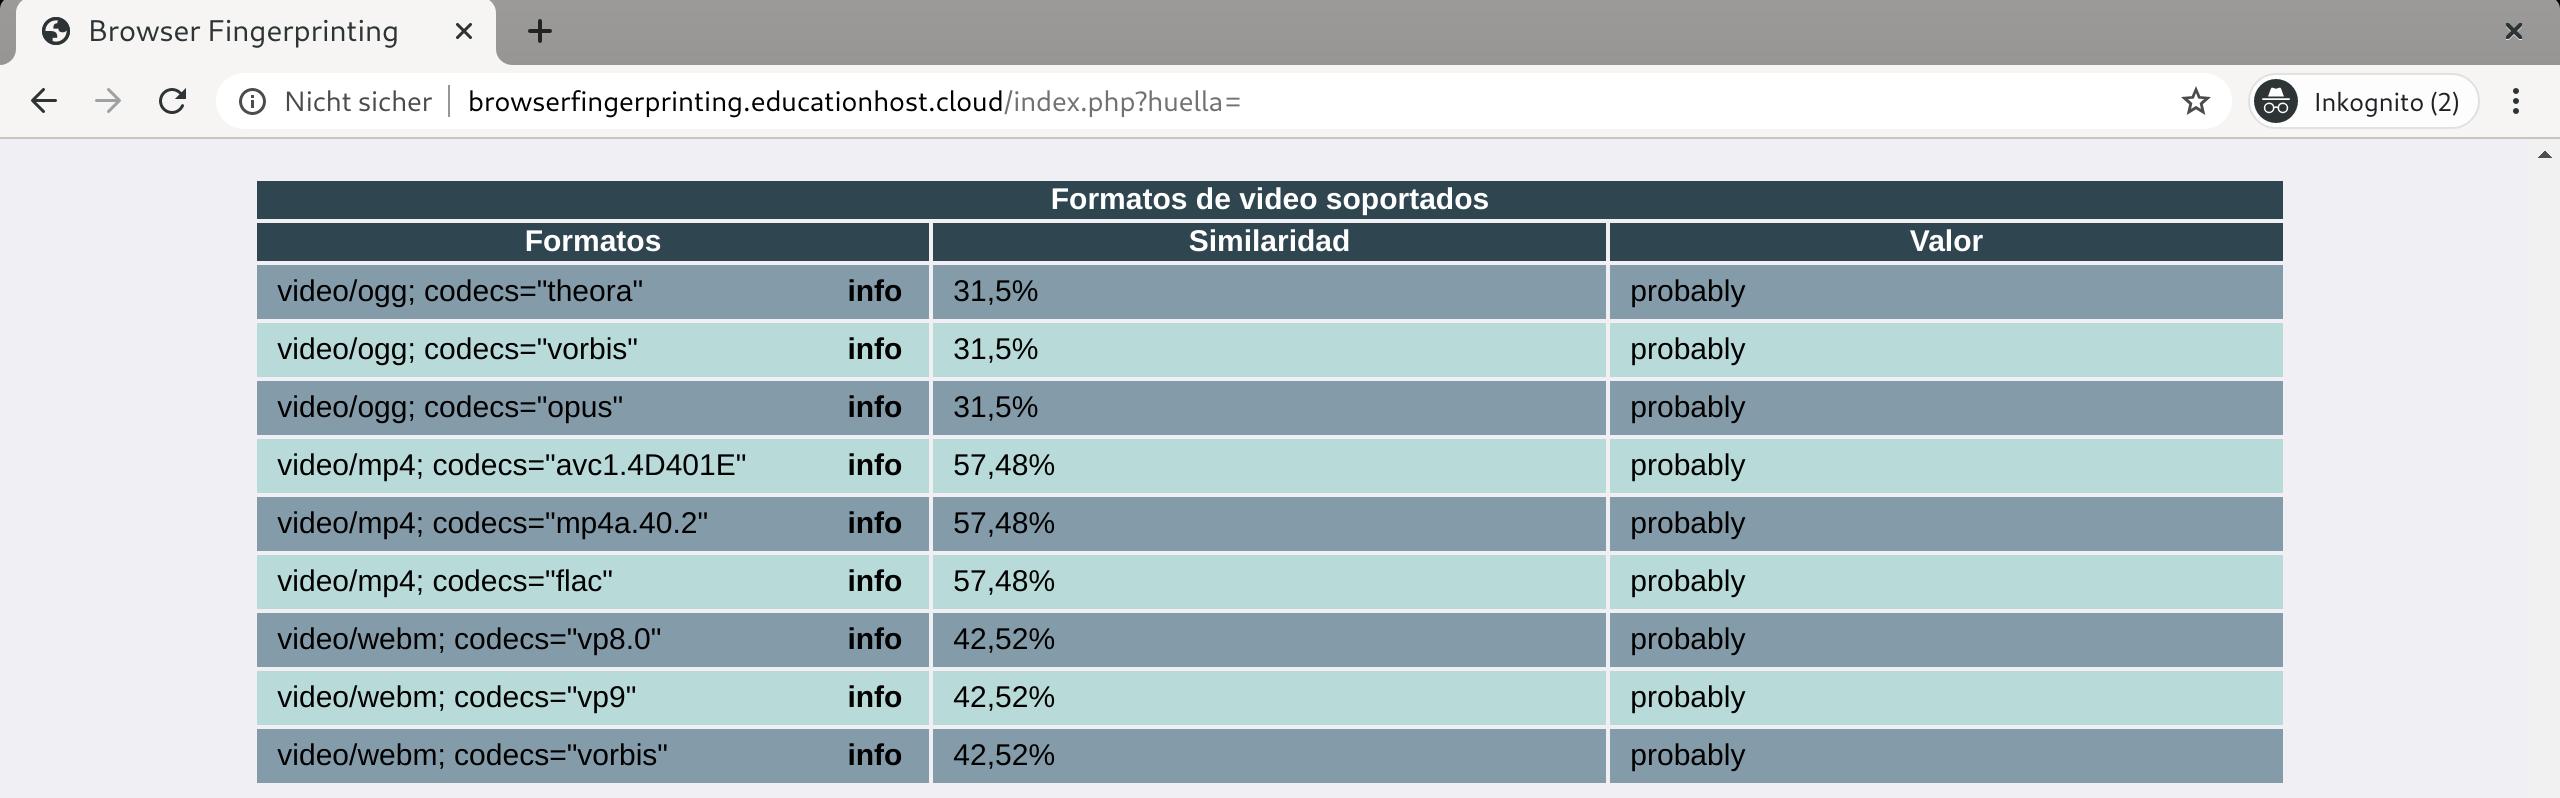
\includegraphics[width=1\textwidth]{Images/videosSection.png}
	\caption{Formatos de vídeo soportados.}
	\label{fig:videosSection}
\end{figure}

\begin{figure}[tbp]
	\centering
	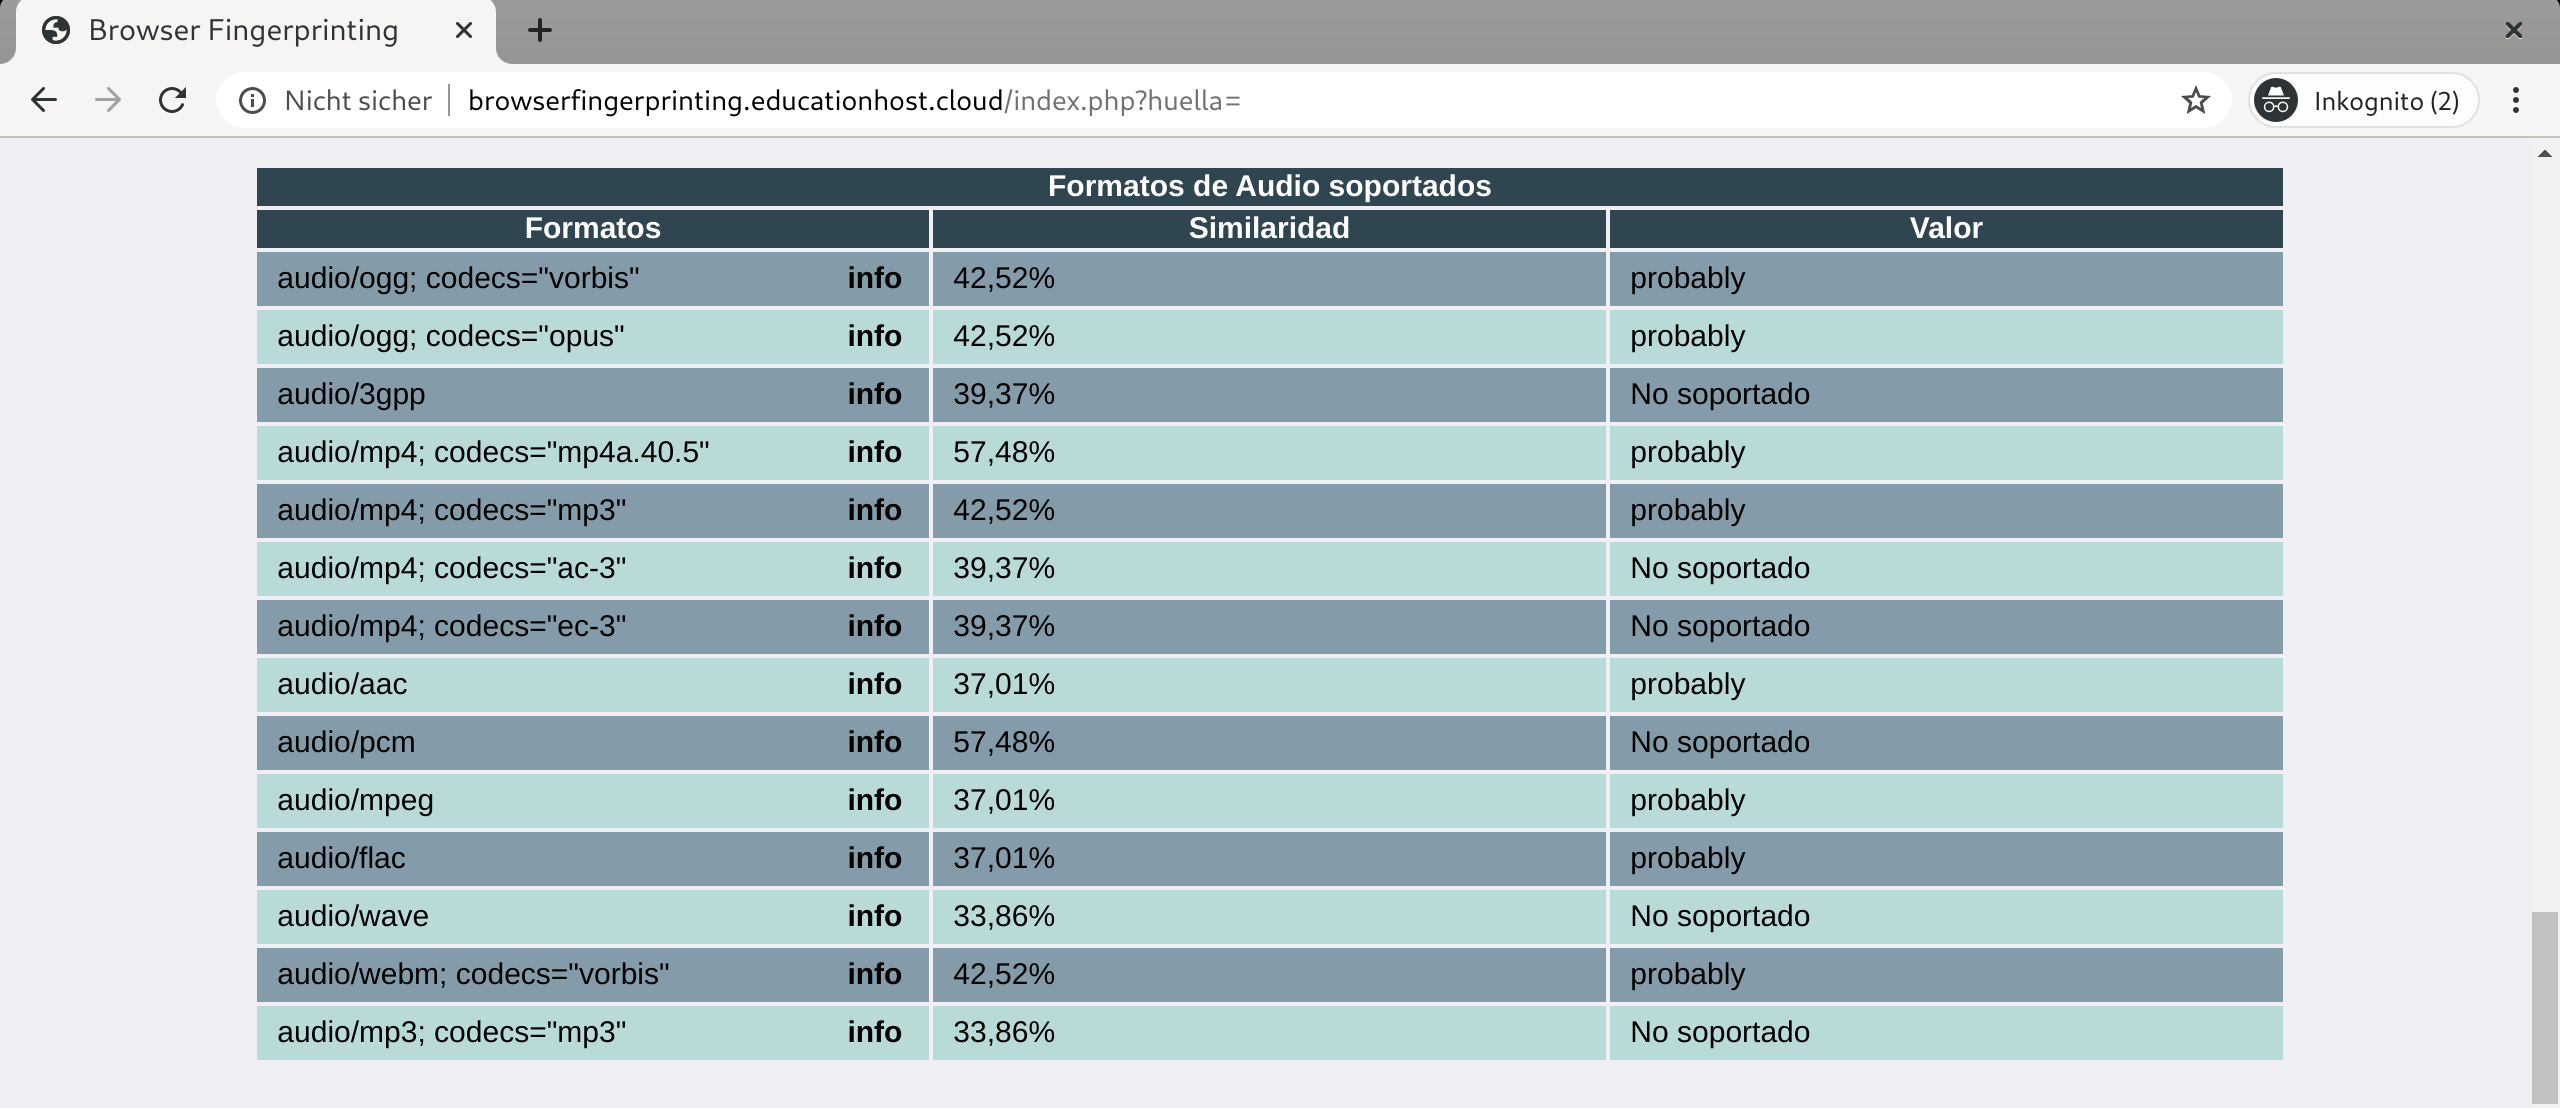
\includegraphics[width=1\textwidth]{Images/audiosSection.png}
	\caption{Formatos de audio soportados.}
	\label{fig:audiosSection}
\end{figure}

\subsubsection{\textit{Plugins}}
En este apartado se recopilan los nombres de las distintas extensiones que hay instaladas en el navegador del cliente. En la tabla de \textit{Plugins}, correspodiente a la figura \ref{fig:pluginsSection}, mostramos también información acerca de los complementos Flash y AdBlock en caso de que estén instalados.

\subsubsection{Fuentes}
En la figura \ref{fig:fuentesSection} se indican cuáles son las fuentes que están instaladas en el sistema. También nos indica el número total de fuentes que han sido detectadas.

\begin{figure}[tbp]
	\centering
	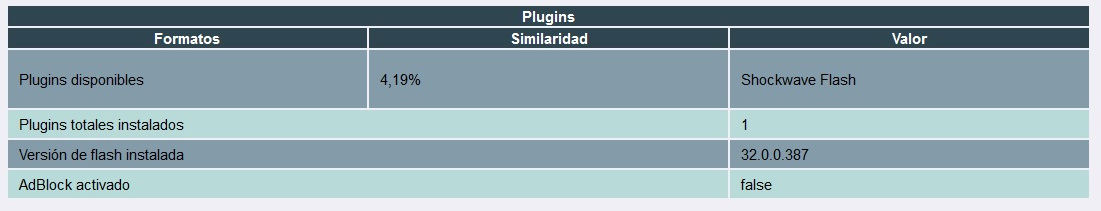
\includegraphics[width=1\textwidth]{Images/pluginsSection.jpg}
	\caption{Información sobre \textit{plugins} del navegador.}
	\label{fig:pluginsSection}
\end{figure}

\begin{figure}[tbp]
	\centering
	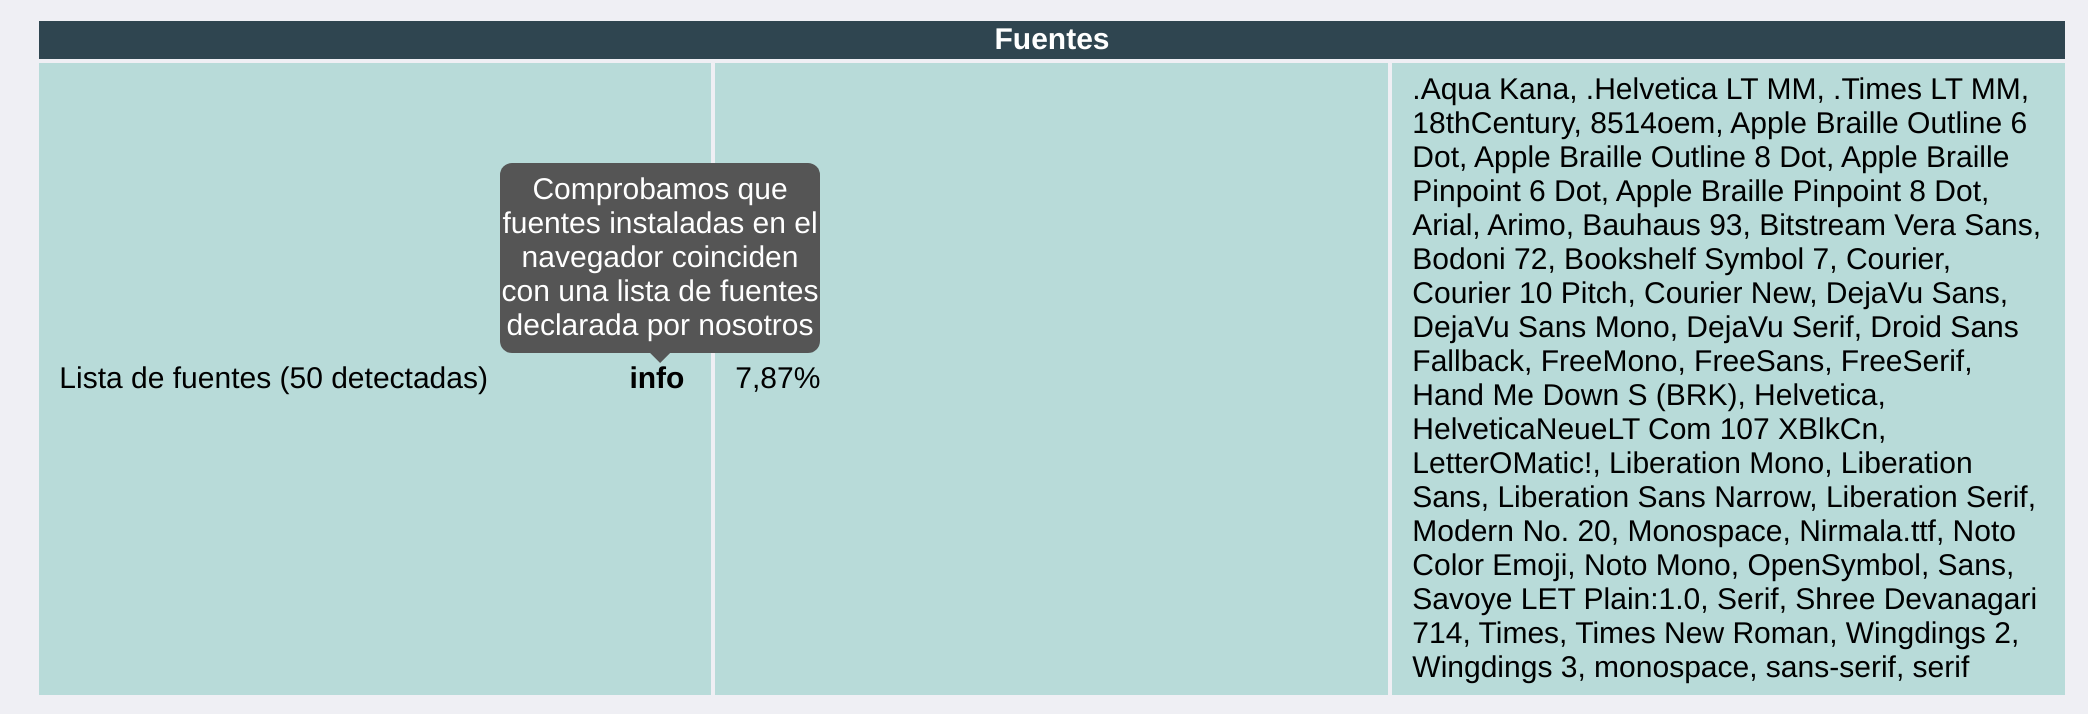
\includegraphics[width=1\textwidth]{Images/fuentesSection.png}
	\caption{Fuentes del navegador.}
	\label{fig:fuentesSection}
\end{figure}

Ya hemos observado las distintas secciones de nuestra tabla con los valores correspondientes. Volveremos a la parte superior de la página y selecionaremos el botón \texttt{Gráficos} para cambiar de ventana (figura \ref{fig:graficosBoton}).

\begin{figure}[tbp]
	\centering
	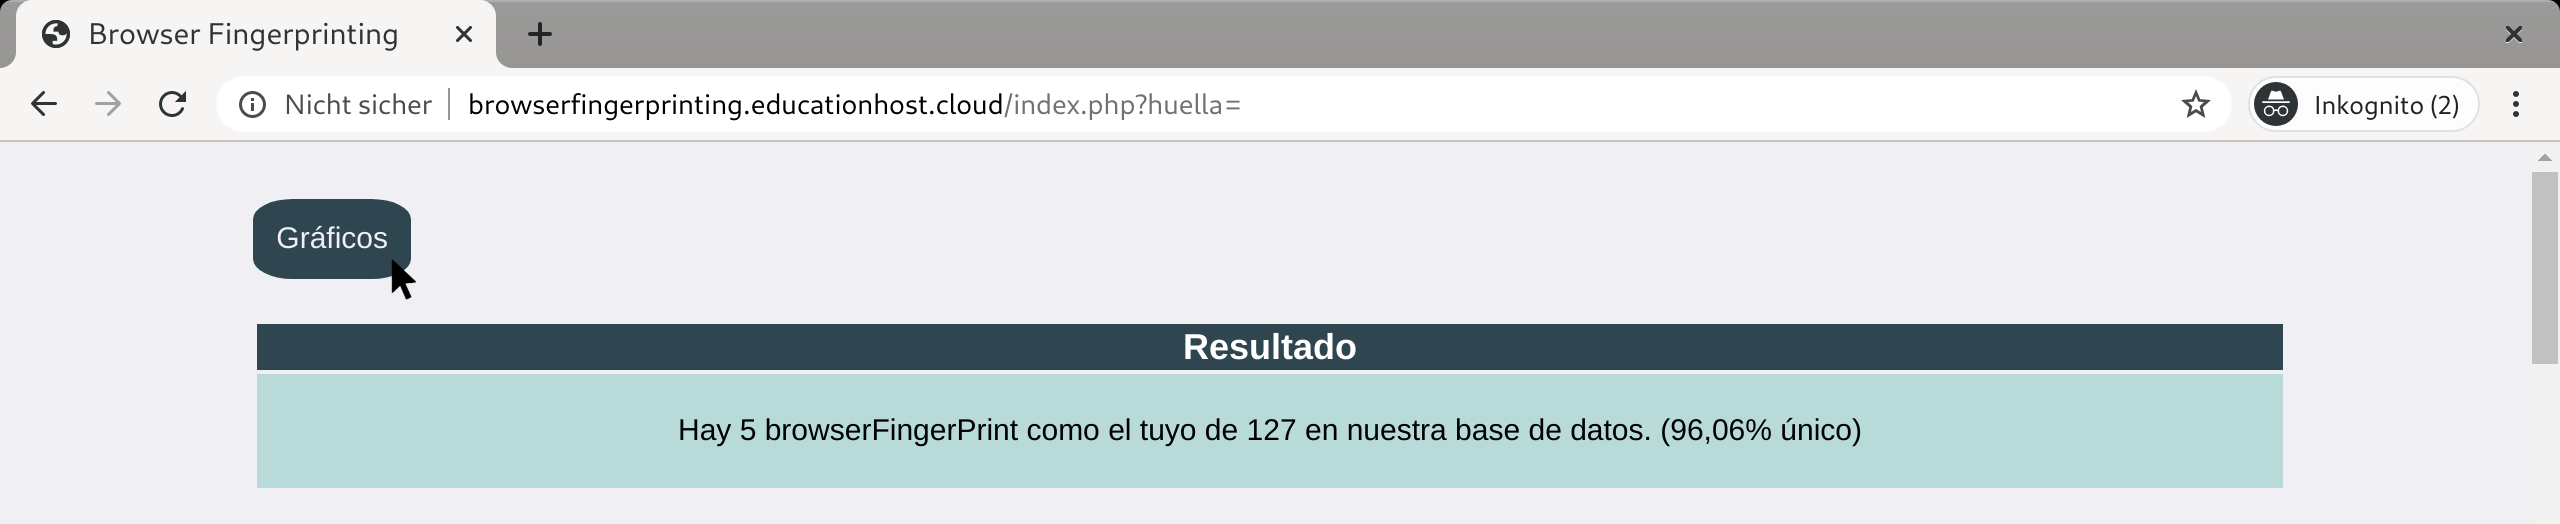
\includegraphics[width=1\textwidth]{Images/graficosBoton.png}
	\caption{Ir a la ventana \texttt{Gráficos}.}
	\label{fig:graficosBoton}
\end{figure}


\section{Gráficos}

Una vez hemos seleccionado el botón \texttt{Gráficos}, aparece en pantalla un gráfico circular en tres dimensiones. 
Este gráfico representa estadísticas para algunos de los parámetros que hemos almacenado en nuestra base de datos. Por defecto, se muestran los porcentajes del atributo \texttt{navegador}. En la figura \ref{fig:navegadorChart} se puede observar la distribución de valores de las conexiones que ha recibido la aplicación. Observamos que a la derecha del gráfico aparece una leyenda de colores que indica cuál es el valor de cada color en el gráfico. 

\begin{figure}[tbp]
	\centering
	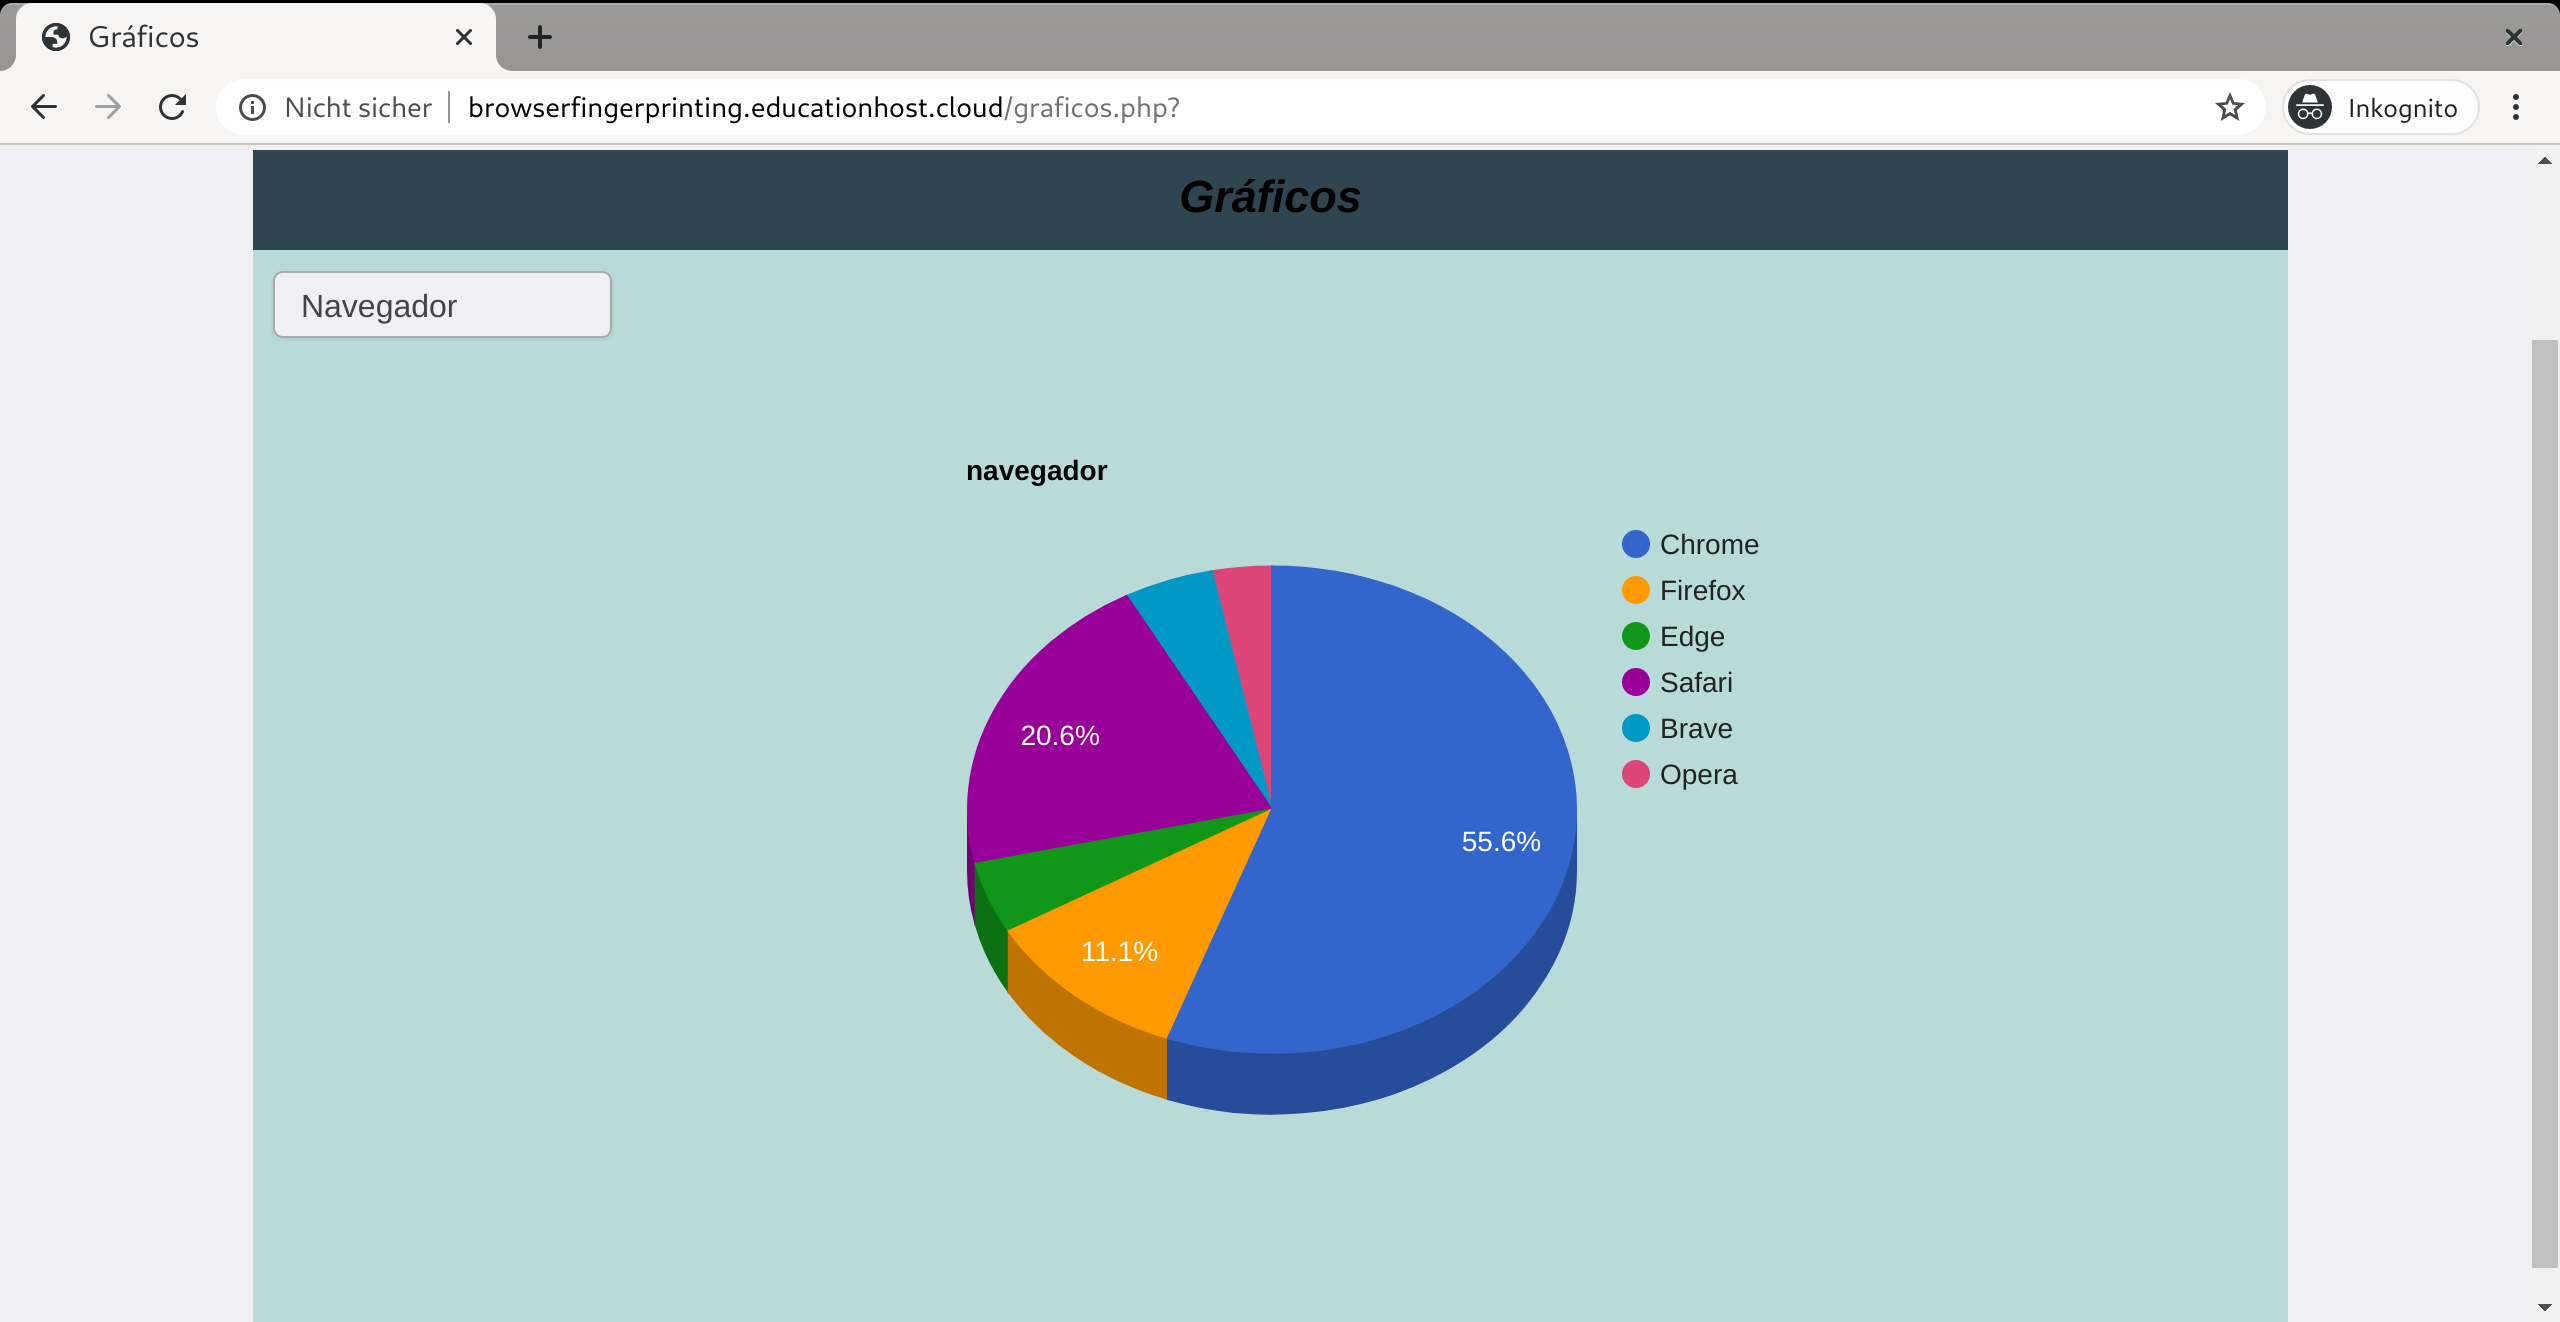
\includegraphics[width=1\textwidth]{Images/navegadorChart.png}
	\caption{Gráfico del atributo \texttt{navegador}.}
	\label{fig:navegadorChart}
\end{figure}

Podemos acceder al menú desplegable que se encuentra arriba a la izquierda. Pinchando sobre el atributo seleccionado, se despliegan las distintas opciones, como se puede ver en la figura \ref{fig:menuChart}. Podemos elegir ver las estadísticas en forma de diagrama de tartas para cada parámetro que se muestra en el menú. En nuestro caso, decidimos ver las estadísticas de \texttt{pixelRatio}, así que seleccionaremos la opción que se muestra en la figura \ref{fig:pixelRatioChart}.

\begin{figure}[tbp]
	\centering
	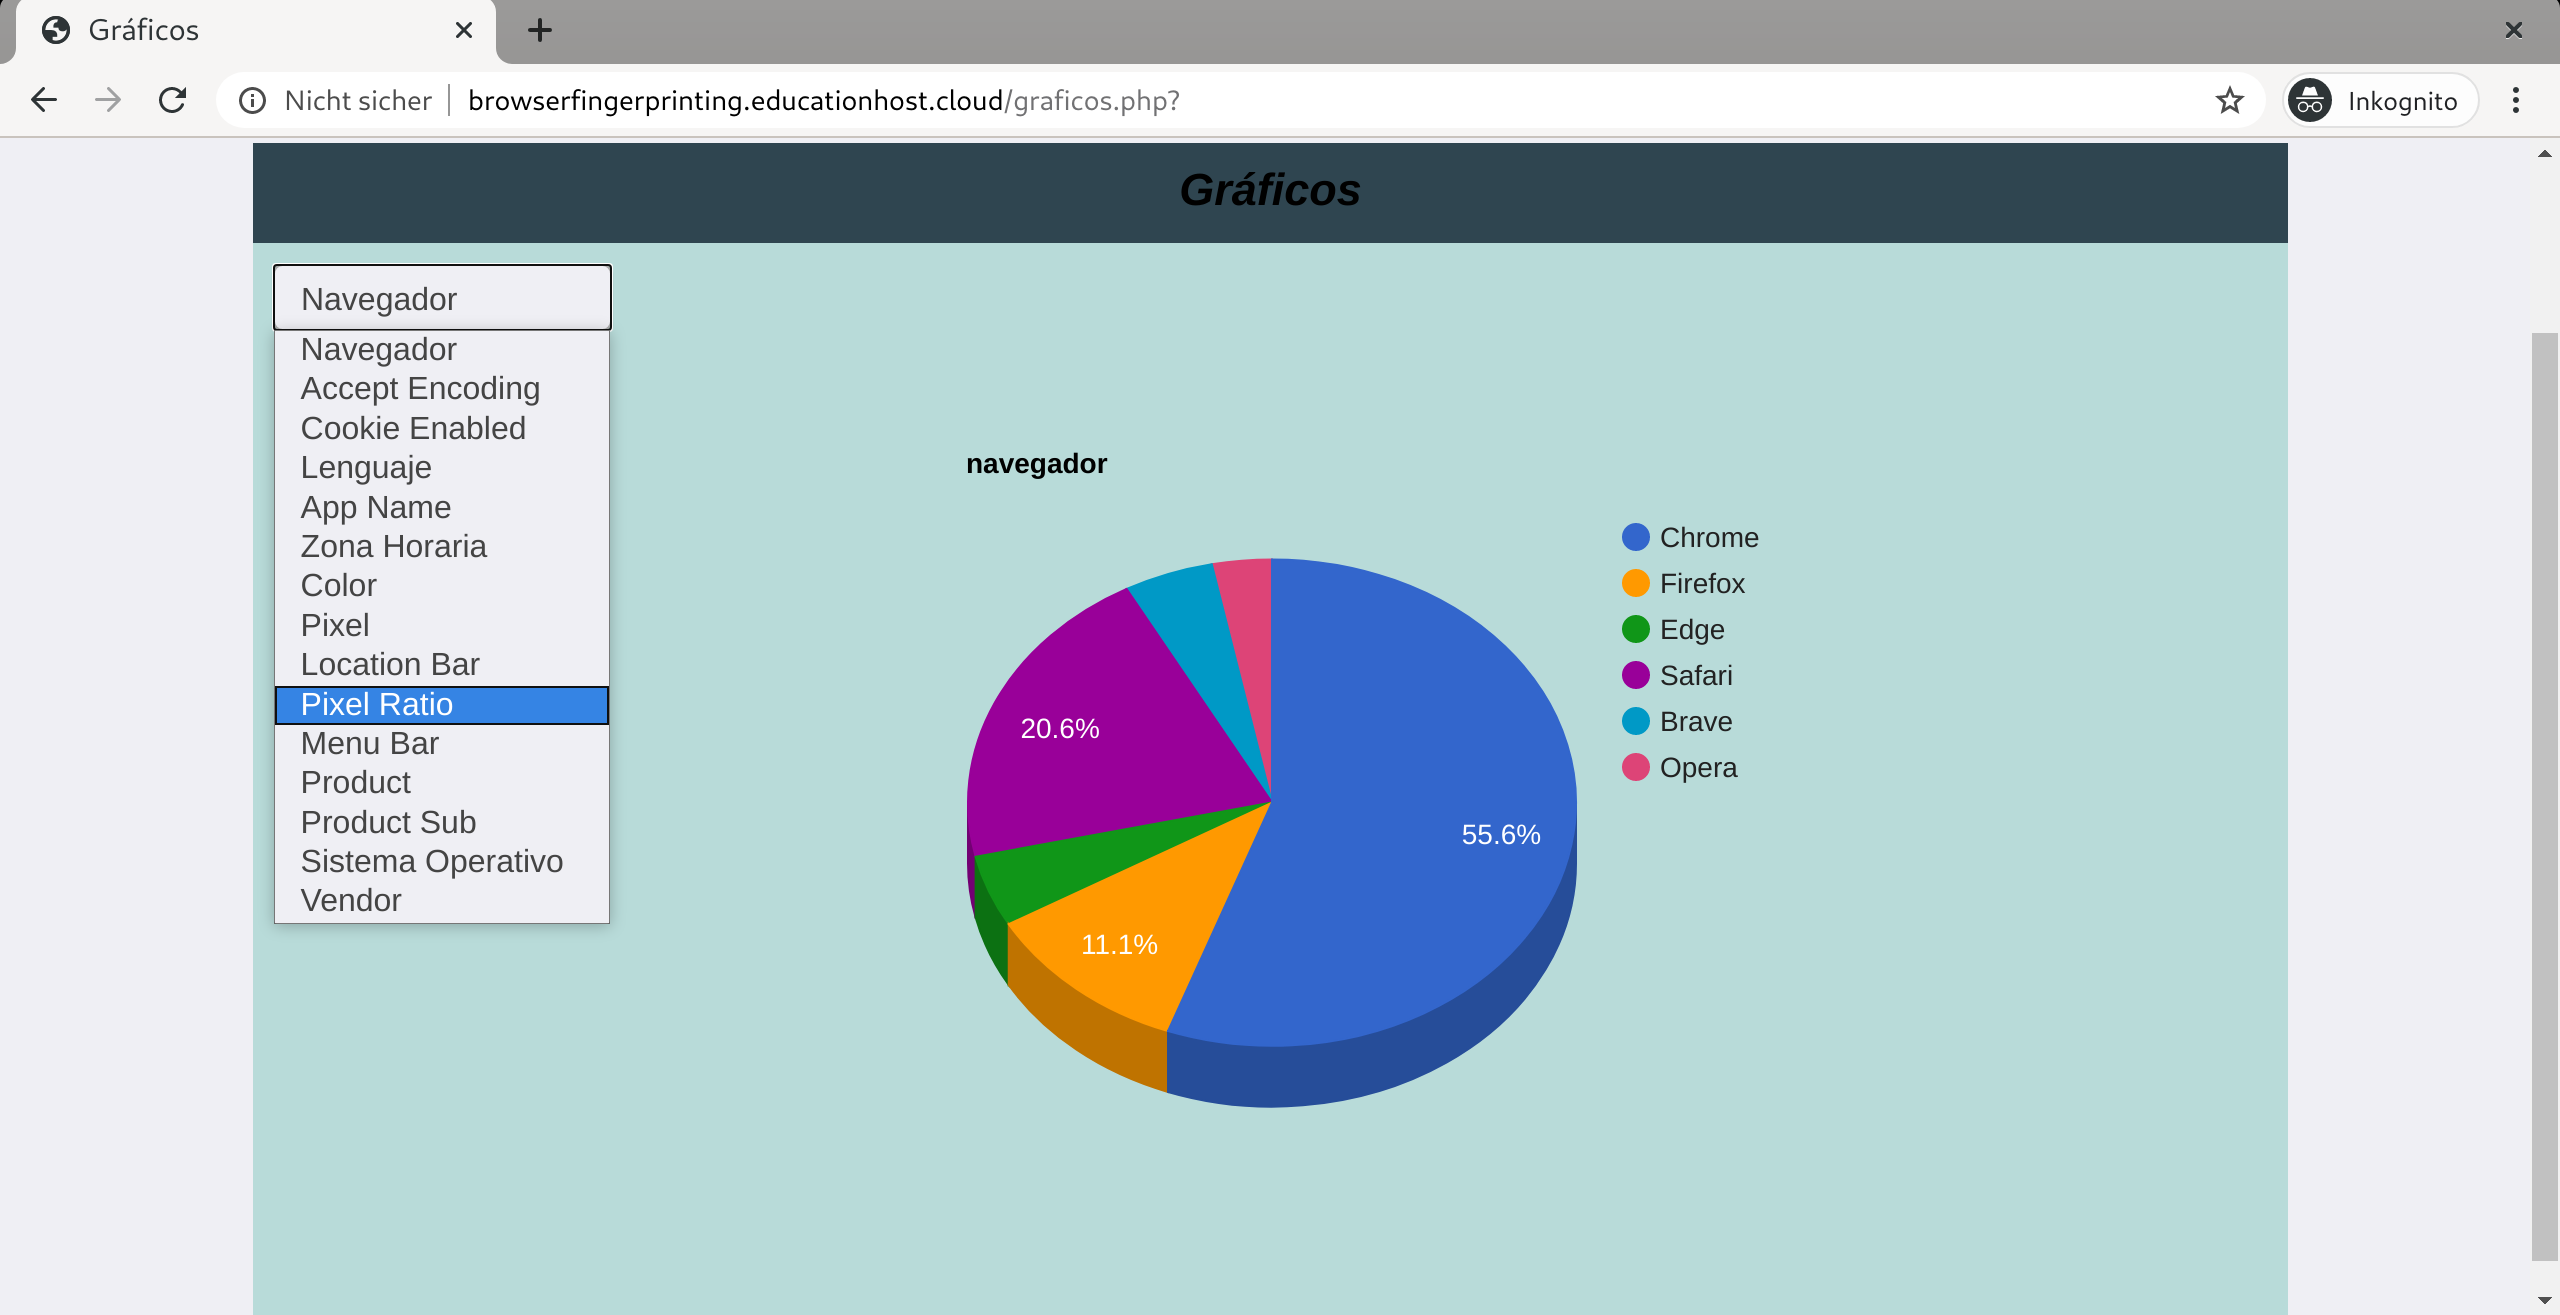
\includegraphics[width=1\textwidth]{Images/menuChart.png}
	\caption{Menú desplegable del apartado de \texttt{Gráficos}.}
	\label{fig:menuChart}
\end{figure}

\begin{figure}[tbp]
	\centering
	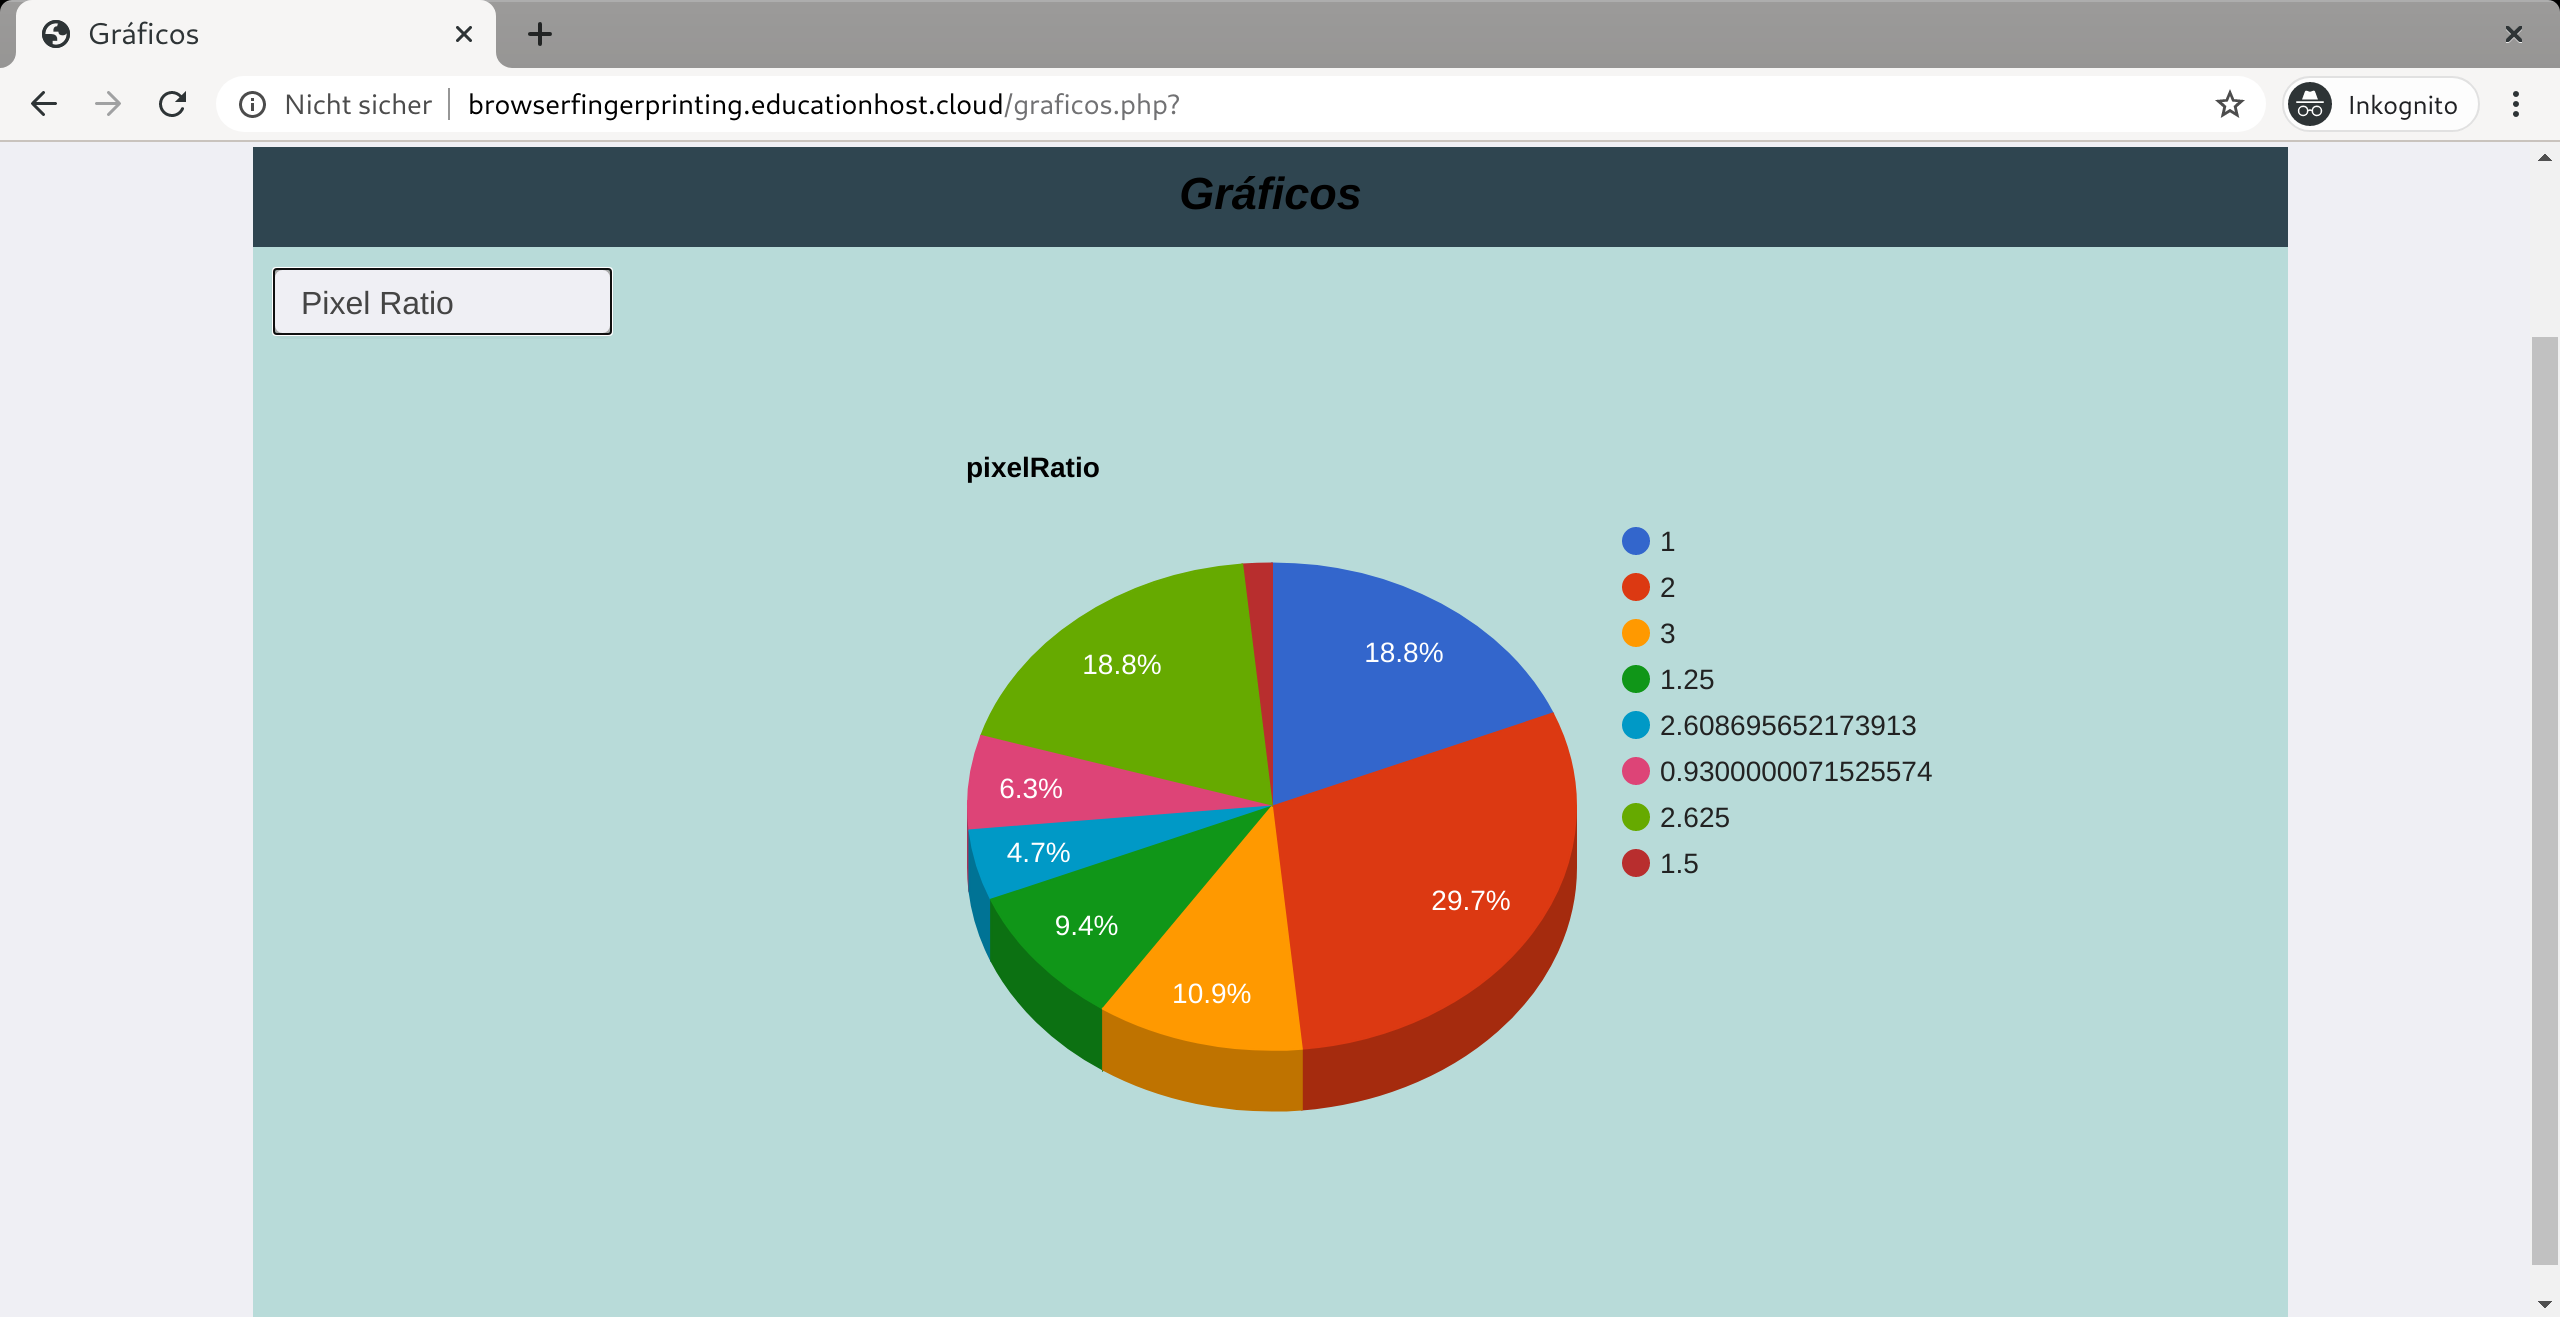
\includegraphics[width=1\textwidth]{Images/pixelRatioChart.png}
	\caption{Gráfico del atributo \texttt{pixelRatio}.}
	\label{fig:pixelRatioChart}
\end{figure}

Las opciones que nos quedan ahora son escoger otro atributo del menú para seguir viendo más diagramas o volver a la pantalla de bienvenida pinchando en el botón \texttt{BrowserFingerprint} de la figura \ref{fig:wellcomeBoton} en la parte superior izquierda de la página.

\begin{figure}[tbp]
	\centering
	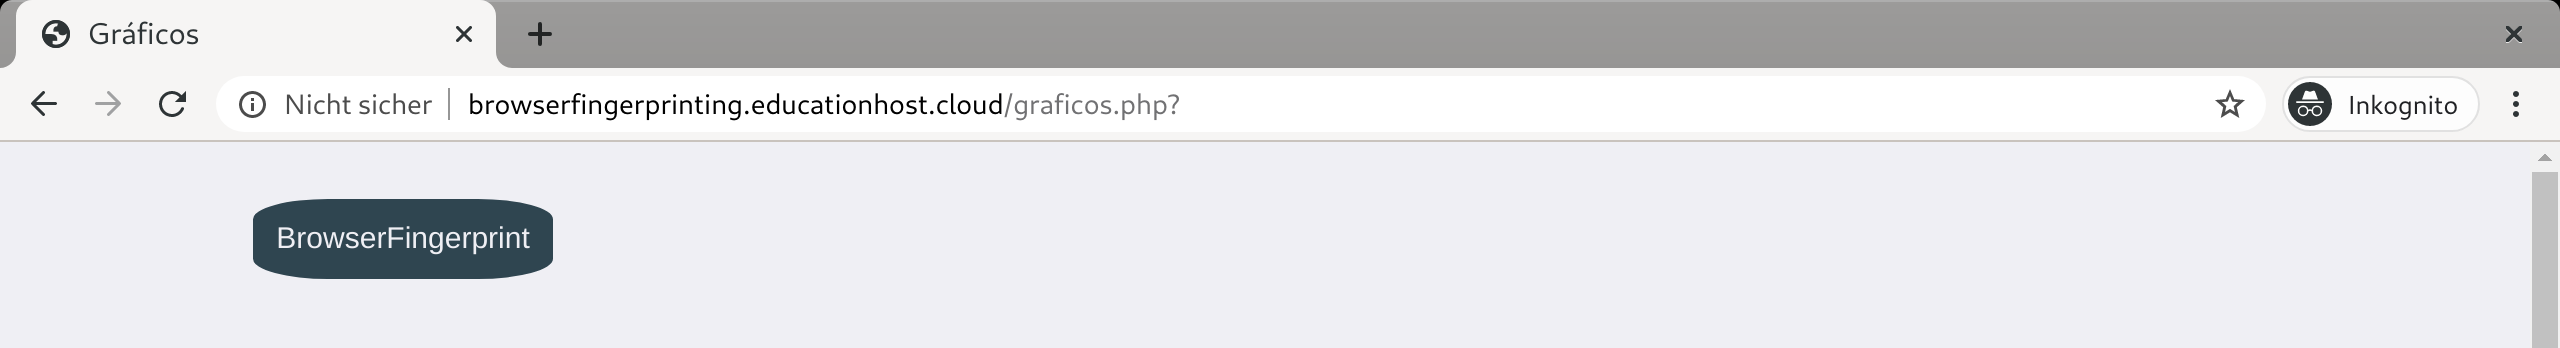
\includegraphics[width=1\textwidth]{Images/wellcomeBoton.png}
	\caption{Volver a la pantalla de bienvenida.}
	\label{fig:wellcomeBoton}
\end{figure}

